\section{Część praktyczna}
\subsection{Subiektywna ocena działania algorytmu}
Celem pierwszej części eksperymetu było zaimplementowanie algorytmu dla gry
w warcaby i subiektywna ocena wybranych przez algorytm posunięć.

Algorytm działał zgodnie z przyjętą heurystyką: różnica sumy wartości własnych
pionków z sumą wartości pionków przeciwnika. Dla głębokości równej 1 zachowanie
komputera można nazwać "zachłannym" - Gdy tylko mógł wykonać bicie, to to
robił. Jednak wielokrotnie samemu poruszał się na pole, z którego mógł zostać
zbity bez możliwości odbicia.

Dla kontrastu, przy głębokości równej 6 jego gra była znacznie lepsza. Ruchy
komputera wydawały się być rozsądne. Niezależnie jednak od tego, czy ruch był
,,naturalnym'' odbiciem jako reakcja na bicie, czy też występował w trudniejszej
do ecenienia pozycji, czas potrzebny na wykonanie ruchu był tak samo długi.


\begin{figure}[h!]
	\centering
	\begin{subfigure}[b]{0.39\linewidth}
		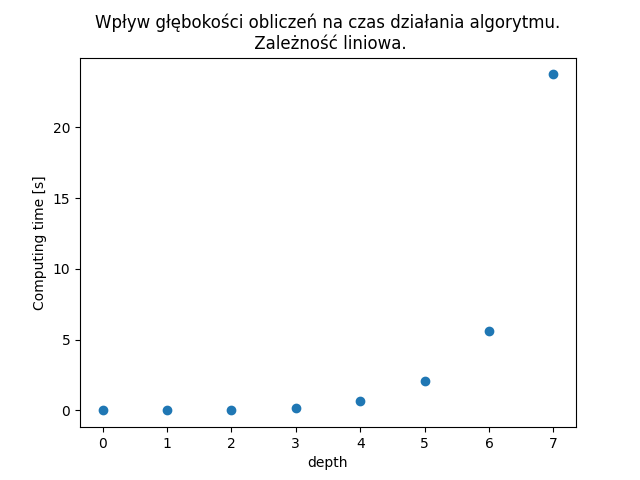
\includegraphics[width=\linewidth]{photos/complexity_linear.png}
		\caption{Wykres liniowy.}
	\end{subfigure}
	\begin{subfigure}[b]{0.39\linewidth}
		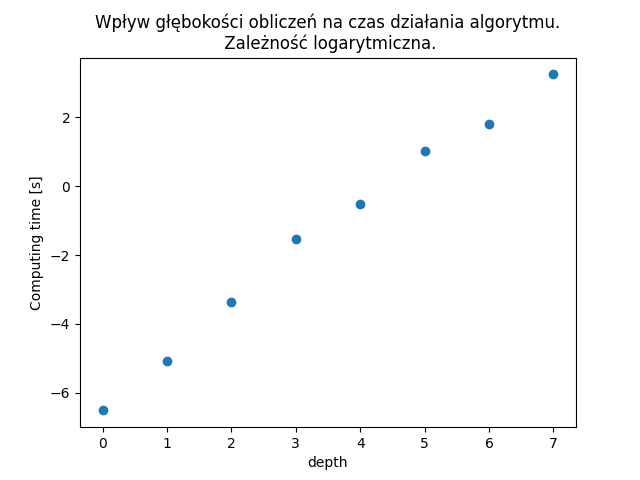
\includegraphics[width=\linewidth]{photos/complexity_logarithmic.png}
		\caption{Wykres logarytmiczny.}
	\end{subfigure}
        \caption{Wykresy złożoności czasowej działania algorytmu w zależności
        od głębokości przeszukiwania.}
\end{figure}


\subsection{Uwagi dotyczące implementacji algorytmu}
\begin{itemize}
    \item Kilkakrotnie podczas testów zaobserwowałem, że w pewnym momencie obaj gracze
    sterowani przez algorytm zaczynały powtarzać posunięcia, co uniemożliwiało
    określenie, który z nich wygrał. Dodatkowo, wywołując algorytm dla takich
    samych parametrów otrzymywałem taki sam przebieg partii. Żeby zmienić te
    rzeczy, mając listę par <ruch, ocena> przed posortowaniem ich ze względu na
    wartość oceny mieszałem je i dopiero wtedy sortowałem. Pozwalało to na wybór
    w tej samej sytuacji innych ścieżek, co zmniejszało monotonny charakter
    rozgrywki.

    \item Głębokość równa 0 została zaimplementowana jako wybór losowego ruchu spośród
dostępnych.

    \item W przypadku heurystyki stosującej ocenę zwartości grupy lub bycie przy
    krawędziach planszy zastosowano następującą interpretację: ,,zwartość'' była
    wyznaczana zarówno poziomo jak i poziomo. Wyliczano ją jako odchylenie
    standardowe liczone dla zbioru położeń (wybranej składowej) wszystkich figur
    danego koloru. Następnie obie sumy (dla poziomu i pionu) sumowano. Zwracano
    różnicę oceny pomiędzy oceną białego a czarnego przeskalowaną o współczynnik.
    Współczynnik wybrano po obserwacji działania algorytmu dla różnych wartości.
    Obecność figury przy krawędzi miało wpływ na ocenę danego piona rzędu 0.1.
\end{itemize}
\subsection{Badanie wpływu głębokości drzewa przeszukiwań oraz rodzaju funkcji
oceny stanu na liczbę wygranych algorytmu}

Celem drugiej części eksperymetu było zbadanie zachowania komputera dla różnych
wartości głębokości drzewa przeszukiwań oraz dla różnych funkcji
heurystycznych, które miały zostać zaimplementowane. 

\begin{table}[htbp!]
    \centering
    \begin{tabular}{ |c|c|c|}
            \hline
            \multicolumn{3}{|c|}{Wpływ głębokości drzewa przeszukiwań oraz rodzaju funkcji oceny} \\
            \multicolumn{3}{|c|}{stanu na liczbę wygranych algorytmu. Badany gracz niebieski.} \\
            \hline
            heurystyka & głębokość & wynik (z perspektywy białego) \\
            ( biały | niebieski ) & ( biały | niebieski ) & (wygrana | remis | przegrana ) \\
            \hline
            \multirow{5}{*}{( default | default )} & ( 2 | 1 ) & ( 6 | 1 | 13 ) \\
            \cline{2-3}
             & ( 2 | 2 ) & ( 0 | 0 | 20 ) \\
            \cline{2-3}
             & ( 2 | 3 ) & ( 0 | 0 | 20 ) \\
            \cline{2-3}
             & ( 2 | 4 ) & ( 1 | 0 | 19 ) \\
            \cline{2-3}
             & ( 2 | 5 ) & ( 0 | 0 | 20 ) \\
            \hline
            \multirow{5}{*}{( default | tight )} & ( 2 | 1 ) & ( 13 | 6 | 1 ) \\
            \cline{2-3}
             & ( 2 | 2 ) & ( 5 | 10 | 5 ) \\
            \cline{2-3}
             & ( 2 | 3 ) & ( 4 | 12 | 4 ) \\
            \cline{2-3}
             & ( 2 | 4 ) & ( 3 | 17 | 0 ) \\
            \cline{2-3}
             & ( 2 | 5 ) & ( 7 | 9 | 4 ) \\
            \hline
            \multirow{5}{*}{( default | enemy side )} & ( 2 | 1 ) & ( 7 | 0 | 13 ) \\
            \cline{2-3}
             & ( 2 | 2 ) & ( 0 | 0 | 20 ) \\
            \cline{2-3}
             & ( 2 | 3 ) & ( 0 | 0 | 20 ) \\
            \cline{2-3}
             & ( 2 | 4 ) & ( 0 | 0 | 20 ) \\
            \cline{2-3}
             & ( 2 | 5 ) & ( 0 | 0 | 20 ) \\
            \hline
            \multirow{5}{*}{( default | hight )} & ( 2 | 1 ) & ( 9 | 1 | 10 ) \\
            \cline{2-3}
             & ( 2 | 2 ) & ( 0 | 0 | 20 ) \\
            \cline{2-3}
             & ( 2 | 3 ) & ( 0 | 0 | 20 ) \\
            \cline{2-3}
             & ( 2 | 4 ) & ( 0 | 0 | 20 ) \\
            \cline{2-3}
             & ( 2 | 5 ) & ( 0 | 0 | 20 ) \\
            \hline
    \end{tabular}
    \caption{Rezultaty pomiarów. Badany gracz niebieski. Parametry gracza białego: głębokość - 2, heurystyka - domyślna.}
\end{table}
Dla domyślnej heurystyki gdy głębokość przeszukiwań niebieskiego wynosiła
więcej niż 1, gracz niebieski niemal zawsze wygrywał.

Zastosowanie heurystyki ,,tight'' skutkowało zwiększaniem się liczby remisów.

Pozostałe heurystyki dawały podobne rezultaty do domyślnej.

\clearpage

\begin{table}[htbp!]
    \centering
    \begin{tabular}{ |c|c|c|}
            \hline
            \multicolumn{3}{|c|}{Wpływ głębokości drzewa przeszukiwań oraz rodzaju funkcji oceny} \\
            \multicolumn{3}{|c|}{stanu na liczbę wygranych algorytmu. Badany gracz: biały.} \\
            \hline
            heurystyka & głębokość & wynik (z perspektywy białego) \\
            ( biały | niebieski ) & ( biały | niebieski ) & (wygrana | remis | przegrana ) \\
            \hline
            \multirow{5}{*}{( default | default )} & ( 1 | 2 ) & ( 0 | 0 | 20 ) \\
            \cline{2-3}
             & ( 2 | 2 ) & ( 0 | 0 | 20 ) \\
            \cline{2-3}
             & ( 3 | 2 ) & ( 0 | 0 | 20 ) \\
            \cline{2-3}
             & ( 4 | 2 ) & ( 0 | 0 | 20 ) \\
            \cline{2-3}
             & ( 5 | 2 ) & ( 0 | 0 | 20 ) \\
            \hline
            \multirow{5}{*}{( tight | default )} & ( 1 | 2 ) & ( 0 | 7 | 13 ) \\
            \cline{2-3}
             & ( 2 | 2 ) & ( 0 | 3 | 17 ) \\
            \cline{2-3}
             & ( 3 | 2 ) & ( 4 | 12 | 4 ) \\
            \cline{2-3}
             & ( 4 | 2 ) & ( 0 | 0 | 20 ) \\
            \cline{2-3}
             & ( 5 | 2 ) & ( 0 | 0 | 20 ) \\
            \hline
            \multirow{5}{*}{( enemy side | default)} & ( 1 | 2 ) & ( 0 | 0 | 20 ) \\
            \cline{2-3}
             & ( 2 | 2 ) & ( 1 | 1 | 18 ) \\
            \cline{2-3}
             & ( 3 | 2 ) & ( 0 | 0 | 20 ) \\
            \cline{2-3}
             & ( 4 | 2 ) & ( 1 | 1 | 18 ) \\
            \cline{2-3}
             & ( 5 | 2 ) & ( 0 | 0 | 20 ) \\
            \hline
            \multirow{5}{*}{( hight | default )} & ( 1 | 2 ) & ( 0 | 0 | 20 ) \\
            \cline{2-3}
             & ( 2 | 2 ) & ( 0 | 0 | 20 ) \\
            \cline{2-3}
             & ( 3 | 2 ) & ( 0 | 0 | 20 ) \\
            \cline{2-3}
             & ( 4 | 2 ) & ( 0 | 0 | 20 ) \\
            \cline{2-3}
             & ( 5 | 2 ) & ( 0 | 0 | 20 ) \\
            \hline
    \end{tabular}
    \caption{Rezultaty pomiarów. Badany gracz biały. Parametry graczaj niebieskiego: głębokość - 2, heurystyka - domyślna.}
\end{table}

Pomimo tego, że głębokość białego zmieniała się od wartości 1 do 5, podczas gdy
głębokość niebieskiego pozostawała stała równa 2, dla każdej heurystyki poza
heurystyką ,,tight'', to niebieski wygrywał większość partii. Przeprowadzenie
badania dla większej wartości głębokości białego nie było możliwe z uwagi na
czas potrzebny na wykonanie testów.

\clearpage

W związku z powyższym przeprowadzono jeszcze jeden test. W stosunku do
poprzedniego zmieniła się w nim tylko jedna rzecz: głębokość niebieskiego
została zmieniona na wartość 1.

\begin{table}[htbp!]
    \centering
    \begin{tabular}{ |c|c|c|}
            \hline
            \multicolumn{3}{|c|}{Wpływ głębokości drzewa przeszukiwań oraz rodzaju funkcji oceny} \\
            \multicolumn{3}{|c|}{stanu na liczbę wygranych algorytmu. Badany gracz: biały.} \\
            \hline
            heurystyka & głębokość & wynik (z perspektywy białego) \\
            ( biały | niebieski ) & ( biały | niebieski ) & (wygrana | remis | przegrana ) \\
            \hline
            \multirow{5}{*}{( default | default )} & ( 1 | 2 ) & ( 9 | 0 | 11 ) \\
            \cline{2-3}
             & ( 2 | 2 ) & ( 7 | 0 | 13 ) \\
            \cline{2-3}
             & ( 3 | 2 ) & ( 9 | 0 | 11 ) \\
            \cline{2-3}
             & ( 4 | 2 ) & ( 9 | 0 | 11 ) \\
            \cline{2-3}
             & ( 5 | 2 ) & ( 11 | 0 | 9 ) \\
            \hline
            \multirow{5}{*}{( tight | default )} & ( 1 | 2 ) & ( 0 | 5 | 15 ) \\
            \cline{2-3}
             & ( 2 | 2 ) & ( 0 | 1 | 19 ) \\
            \cline{2-3}
             & ( 3 | 2 ) & ( 0 | 0 | 20 ) \\
            \cline{2-3}
             & ( 4 | 2 ) & ( 0 | 0 | 20 ) \\
            \cline{2-3}
             & ( 5 | 2 ) & ( 0 | 0 | 20 ) \\
            \hline
            \multirow{5}{*}{( enemy side | default )} & ( 1 | 2 ) & ( 10 | 0 | 10 ) \\
            \cline{2-3}
             & ( 2 | 2 ) & ( 14 | 0 | 6 ) \\
            \cline{2-3}
             & ( 3 | 2 ) & ( 8 | 0 | 12 ) \\
            \cline{2-3}
             & ( 4 | 2 ) & ( 16 | 0 | 4 ) \\
            \cline{2-3}
             & ( 5 | 2 ) & ( 9 | 1 | 10 ) \\
            \hline
            \multirow{5}{*}{( hight | default )} & ( 1 | 2 ) & ( 10 | 0 | 10 ) \\
            \cline{2-3}
             & ( 2 | 2 ) & ( 8 | 0 | 12 ) \\
            \cline{2-3}
             & ( 3 | 2 ) & ( 9 | 0 | 11 ) \\
            \cline{2-3}
             & ( 4 | 2 ) & ( 6 | 0 | 14 ) \\
            \cline{2-3}
             & ( 5 | 2 ) & ( 12 | 1 | 7 ) \\
            \hline
    \end{tabular}
    \caption{Rezultaty pomiarów. Badany gracz biały. Parametry graczaj niebieskiego: głębokość - 1, heurystyka - domyślna.}
\end{table}

Zmniejszenie wartości głębokości niebieskiego spowodowało, że biały częściej
wygrywał dla każdej heurystyki innej od ,,tight''. 

Dla pozostałych heurystyk nie widać wpływu głębokości działania algorytmu na
rezultaty białego. Niezależnie od przyjętej głębi biały wygrywa około połowę
partii pomimo tego, że w niektórych przypadkach głebokość jego obliczeń jest
większa nawet o 4 w porównaniu do niebieskiego gracza.

